\documentclass[18pt]{beamer}
\usepackage{templates/beamerthemekit}
\titlelogo{empty_logo}

\titleimage{my_intro}

\title[Data engineering for astroparticle physics]{Data engineering for joint analysis of different astroparticle data in GRADLC project}
\subtitle{Big Data Science in Astroparticle Research, Aachen University}
\author[Victoria Tokareva]{
  Victoria Tokareva for GRADLC Consortium ~\textbar~18-20 February 2019
}

\institute{Institute for Nuclear Physics (IKP)}

\date{February 20, 2019}

% Bibliography

\usepackage[citestyle=authoryear,bibstyle=numeric,hyperref,backend=biber]{biblatex}
\addbibresource{templates/example.bib}
\bibhang1em

\setbeamertemplate{navigation symbols}{}
\setbeamercovered{invisible}
\usepackage{tikz}
\newcommand{\itemarrow}{\scriptsize\raise1.25pt\hbox{\textcolor{kit-green100}{$\blacktriangleright$}}}
% \newcommand{\itemarrow}{\scriptsize\raise1.25pt\hbox{\textcolor{kit-blue30}{$\blacktriangleright$}}}
\newcommand{\concl}[1]{\item[\itemarrow]\textcolor{kit-green100}{#1}}
\renewcommand{\emph}[1]{\textcolor{kit-green100}{\textbf{#1}}}
\renewcommand{\thefootnote}{\fnsymbol{footnote}}
\newlength{\cellwidth}
\setlength{\cellwidth}{0.43\textwidth}
\newcommand{\cellbox}[1]{\parbox{\cellwidth}{\vspace{1ex}#1\vspace{1ex}}}
\newcommand{\insimg}[1]{
\begin{tikzpicture}[remember picture,overlay]
  \node[xshift=-7.7ex,yshift=12ex] at (current page.south east){%
    \includegraphics[width=14ex]{pics/#1}
  };
\end{tikzpicture}
}

\begin{document}
\selectlanguage{english}

%INTRODUCTION

%title page
\begin{frame}
\titlepage
\end{frame}

\section{Introduction}

\begin{frame}{Big data in astroparticle physics (APP)}
    \small
    \begin{minipage}[c]{0.58\textwidth}
        \begin{center}
            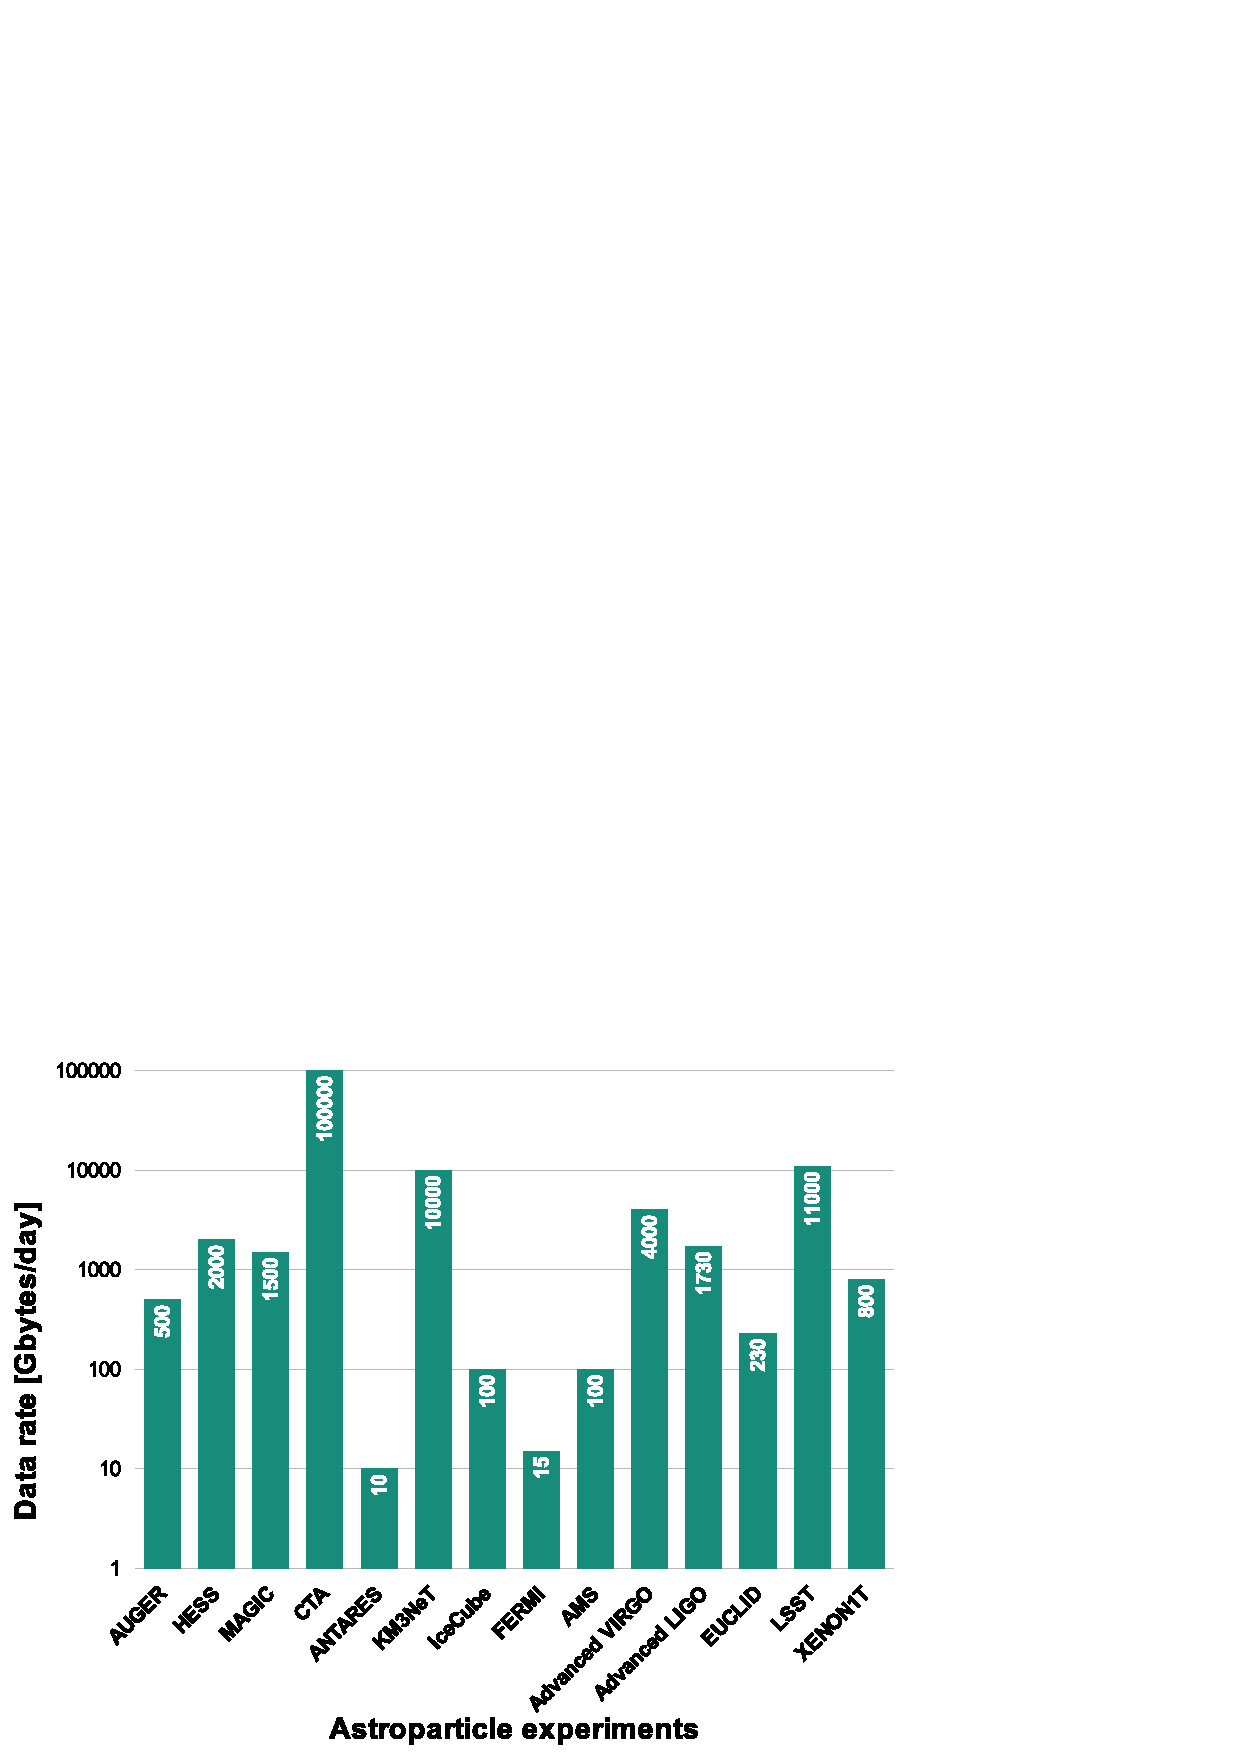
\includegraphics[width=1\textwidth]{pics/appec_computing-diagram.pdf}
        \end{center}
        \vspace{-2\parsep}
        \small Modern astroparticle experiments data rate [Gbytes/day]\footnotemark[1] %, source: APPEC brochure on Computing, 2016}
    \end{minipage}
    \hfill
    \begin{minipage}[c]{0.41\textwidth}
        \begin{itemize}
            \setlength{\itemsep}{0pt}
            \item Wide range of experiments;
            \item More than hundred years of cosmic particle measurements;
            \item Looking at the same sky with different detectors;
            \item Common data rate for astropartical physics experiments all together is a few PBytes/yeary, which is comparable to the current LHC output\footnotemark[1]
            \item Big data for deep learning
        \end{itemize}
    \end{minipage}
    \footnotesize\footnotetext[1]{Berghöfer T., Agrafioti I. et all. Towards a model for computing in European astroparticle physics, Astroparticle Physics European Coordination committee, 2016}
\end{frame}

\begin{frame}{Software data life cycles}% and information management
    \begin{itemize}
        \item \textbf{Data engineering} includes development and support of data architecture and a data pipeline for a data platform that enables data analysts, scientists, and other personnel to query the data.
        % and organization and support of a data pipeline that connects all the pieces of the data ecosystem together.
        
        \item \textbf{Data Life Cyce (DLC)} is the sequence of stages that a particular unit of data goes through from its initial generation 
        or capture to its eventual archival and/or deletion. The typical data life cycle includes data gathering, processing, storage, analysis, sharing and archiving. 
        % The data life cycle provides a high level overview of the stages involved in successful management and preservation of data for use and reuse.

        % \item \textbf{Data engineering} includes development of the architecture for a data platform that enables data analysts, scientists, and other curious 
        %  types to query their data and organization and support of a data pipeline that connects all the pieces of the data ecosystem together.
        %  
        %  \item \textbf{Data Life Cyce (DLC)} is the sequence of stages that a particular unit of data goes through from its initial generation 
        % or capture to its eventual archival and/or deletion. The typical data life cycle includes data gathering, processing, storage, analysis, sharing and archiving. The data life cycle provides a high level overview of the stages involved in successful management and preservation of data for use and reuse.
    \end{itemize}
    \vspace{-1ex}
    \centering
    \includegraphics[width=0.65\textwidth]{pics/data_lifecycle_illust.jpg}
\end{frame}

%contents
\begin{frame}{Data engineering in APP}

\begin{minipage}[c]{0.52\textwidth}
\small
  \begin{itemize}
      \setlength{\itemsep}{0pt}
%       \item  Introduction \textcolor{kit-green100}{$\rightarrow$ we are here}
      \item  GRADLC initiative and main objectives
      \item  Features of DLC in APP
      \item  KASCADE Cosmic-ray Data Center
      \item  Proposed DCL architecture
      \item  Data aggregation server: metadata, data summary and workflows
%       \begin{itemize}
% 	  \item Metadata architecture
% 	  \item Data workflows 
% 	  \item Data summary and challenges (no slide so far :-( )
% 	  \item Possible solutions (postgres, cvmfs, etc...)
%       \end{itemize}
      \item   Application server: conception, computing sources and analysis
%       \begin{item}
% 	  \item conception 
% 	  \item computing sources
% 	  \item analysis 
% 	  \item possible solutions
%       \end{item}

      \item  Example: stacked analysis of high-energetic gamma rays
      \item  Outlook

%     \item  DCL in APP - specific
%     \item  DCL architecture
%     \item  Experiments and data specific
%     \item  Joint analysis scheme
%     \item  Possible solutions
%     \item  Outlook and future work
  \end{itemize}
\end{minipage}
\hfill
\begin{minipage}[c]{0.47\textwidth}
  \includegraphics[width=1\textwidth]{pics/DE_fun.pdf}
\end{minipage}
\end{frame}

%GRADLC initiative descripton 

\begin{frame}{German-Russian Astroparticle \\Data Life Cycle Initiative\footnotemark[1]}
\vspace{-1.4em}
\begin{center}
  \includegraphics[width=0.9\textwidth]{pics/Collab-4.pdf}
\end{center}
\footnotesize\footnotetext[1]{Granted by RSF-Helmholtz Joint Research Groups}
\end{frame}

% %experiments overview

\begin{frame}{KASCADE-Grande}
\begin{itemize}
  \item Proposed in 1989---disassembled in 2013;
  \item Aimed at studying
  high-evergy (galactic) cosmic rays by observing extensive air showers (EAS);
%   processes at the edge of the Galaxy and beyond by observing extended atmospheric showers (EAS);
  \item Consisted of:
  \begin{itemize}
    \item scintillator arrays:
%     detecting $e$, $\gamma$, $\mu$:
    \begin{itemize}
  %сцинтиляторы, различают e, gamma, mu
    \item KASCADE---256 stations;
    \item GRANDE---37 stations;
    \end{itemize}
 %один большой калориметр
    \item Hadronic callorimeter;
 %радиодетектор
    \item Digital radio array LOPES;
%     detecting $e$, $e^{+}$;
% позволяющих наблюдать различные компоненты ливня
  \end{itemize}
  \item Important features of cosmic-ray spectrum have been obtained. The data analysis is ongoing;
%  благодаря данным с эксперимента было открыто много всего ополезного, при этом анлиз данных продолжается. новые статьи выходят
  \item KCDC (\textbf{K}ASCADE \textbf{C}osmic Ray \textbf{D}ata \textbf{C}enter, \textcolor{blue}{\texttt{http://kcdc.ikp.kit.edu}}) is a dedicated portal where all the data collected are available online. % At the moment
\end{itemize}

\begin{tikzpicture}[remember picture,overlay]
  \node[xshift=-12ex,yshift=-21ex] at (current page.north east){%
    \includegraphics[width=0.3\textwidth]{pics/KCDC-Logo.png}
  };
\end{tikzpicture}
\end{frame}

\begin{frame}{TAIGA---Tunka Advanced Instrument for \mbox{cosmic ray physics and Gamma Astronomy}}
\vspace{-1em}
\begin{itemize}
 \item Started in the mid 90s, is still operating and continiously enhancend
%  \item Currently consists of 4 detectors presented + TUNKA IACT is under construction;
\end{itemize}
\footnotesize
\vspace{-2em}
\begin{minipage}[t]{0.31\textwidth}
  \begin{block}{\small Tunka-133}
    \parbox[c][0.20\textheight][t]{1\textwidth}{
      \centering
      \includegraphics[width=0.7742\textwidth]{pics/Tunka-133.jpg}
    }
    \hfill
    \parbox[c][0.15\textheight][t]{1\textwidth}{
      \begin{itemize}
        \setlength{\itemsep}{0pt}
        \item 133 photomultipliers
        \item measures EAS Cherenkov light
      \end{itemize}
    }
  \end{block}
\end{minipage}
\hfill
\begin{minipage}[t]{0.31\textwidth}
  \begin{block}{\small Tunka-Rex}
    \parbox[c][0.20\textheight][t]{1\textwidth}{
      \centering
      \includegraphics[width=0.7742\textwidth]{pics/Tunka-Rex.jpg}
    }
    \\
    \parbox[c][0.15\textheight][t]{1\textwidth}{
      \begin{itemize}
        \setlength{\itemsep}{0pt}
        \item 63 antennas
        \item measures EAS radio-emission
      \end{itemize}
    }
  \end{block}
\end{minipage}
\hfill
\begin{minipage}[t]{0.31\textwidth}
  \begin{block}{\small Tunka-HiSCORE}
    \parbox[c][0.20\textheight][t]{1\textwidth}{
      \centering
      \includegraphics[width=0.7742\textwidth]{pics/Tunka-HiSCORE.jpg}
    }
    \\
    \parbox[c][0.15\textheight][t]{1.1\textwidth}{
      \begin{itemize}
        \setlength{\itemsep}{0pt}
        \item 47$\times$4 photomultipliers
        \item measures EAS Cherenkov light
      \end{itemize}
    }
  \end{block}
\end{minipage}

\vspace{-1ex}
\begin{minipage}[t]{0.48\textwidth}
  \begin{block}{\small Tunka-Grande}
    \parbox[c][0.21\textheight][t]{0.43\textwidth}{
      \includegraphics[width=0.50\textwidth]{pics/Hiller_Roman-005.jpg}
    }
    \hfill
    \parbox[c][0.21\textheight][t]{0.55\textwidth}{
      \begin{itemize}
        \setlength{\itemsep}{0pt}
        \item 380 scintillators 0.64m$^2$ each
        \item measures $e$/$\mu$ from EAS
      \end{itemize}
    }
  \end{block}
\end{minipage}
\hfill
\begin{minipage}[t]{0.48\textwidth}
  \begin{block}{\small Tunka-IACT}
    \parbox[c][0.21\textheight][t]{0.43\textwidth}{
      \includegraphics[width=0.50\textwidth]{pics/Tunka-Iact.jpg}
    }
    \hfill
    \parbox[c][0.21\textheight][t]{0.55\textwidth}{
      \begin{itemize}
        \setlength{\itemsep}{0pt}
        \item Imaging Air Cherenkov Telescopes
        \item is being extended
      \end{itemize}
    }
  \end{block}
\end{minipage}
\end{frame}
 - experiments overview. Is not requiered is this IT=specified presentation
% 
% \begin{frame}{The main objectives}
% \begin{minipage}[c]{0.45\textwidth}
%   \begin{itemize}
%     \item  Provide sustainable access to scientific data
%     \item  Archiving of Data and Metadata
%     \item  Providing analysis tools
%     \item  Education in Big Data Science
%   \end{itemize}
% \end{minipage}
% \hfill
% \begin{minipage}[c]{0.54\textwidth}
%   \includegraphics[width=1\textwidth]{pics/proj_objectives.pdf}
% \end{minipage}
%   \vspace{-\topsep}
%   \vspace{-\partopsep}
%   \vspace{\itemsep}
%   \vspace{\parsep}
%   \begin{itemize}
%     \item  Development area for multi-messenger analyses (e.g. Deep Learning)
%     \item  Platform for communication and exchange within Astroparticle Physics
%   \end{itemize}
% \end{frame}
% 



\section{Data life cycle}
%DLC IN GENERAL:
%DLC development

\begin{frame}{Features of DLC in APP}
    \begin{minipage}[c]{0.64\textwidth}
        \begin{itemize}
            \item Constantly growing precision and data amounts;
            \item Rare events and low statistics;
            \item Call for multi-messenger astrophysics;
            \item Need for various data in analysis;
            \item Data mining in astroparticle data;
            \item Need for advanced storage architectures and smart data selection queries.

        %     \item Experiments improve and are measuring events with greater precision (large amount of data);
        %     \item But not too many events of our interest;
        %     \item[$\Rightarrow$] combined analysis of data from different experiments becomes topical;
        %     \item Astronomical Virtual Observatories (Auger \& IceCube data).


        %     \item  constantly growing precission and data amounts;
        %     \item rare events and low statistics;
        %     \item call for multi-messenger astrophysics;
        %     \item  need for various data in analysis;
        %     \item data mining in astroparticle data;
        %     \item Need for advanced storage architectures and smart data selection queries
        \end{itemize}
    \end{minipage}
    \hfill
    \begin{minipage}[c]{0.35\textwidth}
        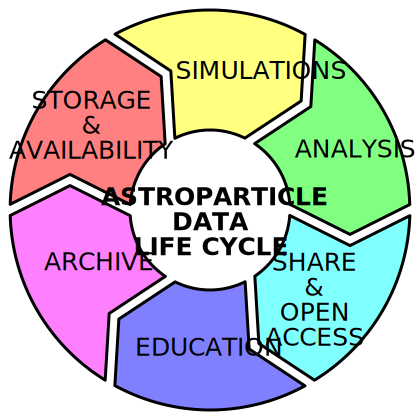
\includegraphics[width=1\textwidth]{pics/ADLC.pdf}
    \end{minipage}
\end{frame}
% 
% \begin{frame}{KASCADE Cosmic-ray Data Center (KCDC) in a nutshell}
%         \tiny
%  \textcolor{red}{the overview is taken from A.Haungs. Rewrite!}
%   \textcolor{red}{Add KCDC logo and scheme!}
%     \begin{itemize}
%              \tiny
%         \item providing open access to astroparticle physics research data
%         as required by funding agencies
%         \begin{itemize}
%             \item data provider
%             \begin{itemize}
%                 \item follows the “Berlin Declaration on Open Data and Open Access”
%                 \item free, unlimited, open access to KASCADE cosmic ray data
%                 \item selection of fully calibrated quantities and detector signals
%                 \item reliable data source
%                 \item guaranteed data quality
%             \end{itemize}
%             \item information platform
%             \begin{itemize}
%                 \item experiment description
%                 \item meta information for data analysis
%                 \item physics background
%                 \item use of modern and open source web technologies
%                 \item tutorials (focused on teachers and pupils)
%             \end{itemize}
%             \item long-term digital data archive
%             \begin{itemize}
%                 \item archive of software and data
%                 \item for the collaboration
%                 \item for the public 
%             \end{itemize}
%         \end{itemize}
%     \end{itemize}
% \end{frame}

\begin{frame}{KASCADE Cosmic-ray Data Center (KCDC)}
    \begin{itemize}
        \small
        \setlength{\itemsep}{0pt}
        \item providing free, unlimited, reliable open access to KASCADE cosmic ray data at \textcolor{blue}{\underline{https://kcdc.ikp.kit.edu}};
        \item almost all KASCADE data is available;
        \item selection of fully calibrated quantities and detector signals;
        \item information platform: physics and experiment backgrounds, tutorials, meta information for data analysis;
        \item archive of KASCADE software and data;
        \item uses modern and open source web technologies.
    \end{itemize}

\includegraphics[height=0.35\textheight]{pics/KCDC-Logo.png}
\hfill
\includegraphics[height=0.35\textheight]{pics/KCDC-IT-Structure.pdf}
\end{frame}

\begin{frame}{KASCADE and TAIGA data rates}
\begin{minipage}[c]{0.52\textwidth}
% \small
  \begin{itemize}
    \item KASCADE:
    \begin{itemize}
      \item 450 000 000 events
      \item ~ 4 Tb of measured data
    \end{itemize}
    \vspace{1em}
    \item planned TAIGA rate: ~ 20 TB/year
    \begin{itemize}
      \item HiSCORE: ~ 18 TB/year
      \item IACT: 1.5 TB/year
      \item others: ~ 0.5 TB/year
    \end{itemize}
  \end{itemize}
\end{minipage}
\hfill
\begin{minipage}[c]{0.47\textwidth}
\vspace{-3.5em}
  \begin{itemize}
    \item current TAIGA rate: 
    \begin{itemize}
      \item ~ 50 Tb of raw data;
      \item ~ 8 TB/year of reconstructed data:
      \begin{itemize}
  \item HiSCORE: 6.4 TB/year
  \item IACT: 1 TB/year
  \item others: ~ 0.5 TB/year
      \end{itemize}
    \end{itemize}
  \end{itemize}
\end{minipage}

\end{frame}

\begin{frame}{DLC Architecture}
\begin{minipage}[c]{0.63\textwidth}
  \includegraphics[width=1\textwidth]{pics/arch_appds.png}
\end{minipage}
\hfill
\begin{minipage}[c]{0.36\textwidth}
  \small
  \begin{itemize}
    \setlength{\itemsep}{0pt}
%     \setlength{\parskip}{0pt}
    \item\textbf{Si} — local data storages;
    \item\textbf{Ini} — data sources of different types;
    \item\textbf{MDD} — metadata description;
    \item\textbf{Ei} — metadata extractors;
    \item\textbf{Ai} — adapters, provide API for data access;
    \item\textbf{TPL} — template library;
    \item\textbf{MD DB} — metadata database.
  \end{itemize}
\end{minipage}
\end{frame}

% DATA AGGREGATION SERVER:
% Data aggregation server:

\begin{frame}{Requirements for the data warehouse}
  \begin{itemize}
    \item Multiple experiments (TAIGA, KASCADE, etc.)
    \item More than hundreds of terabytes of raw data at each site
    \item Remote access to query results as local file systems
    \item  On-demand data transfer by requests only
    \item  Automatic real-time updates
    \item  No changes to existing site infrastructure, only add-ons
  \end{itemize}
\end{frame}

\begin{frame}{Proposed solution for data aggregation}
\textbf{Main solution components}: CVMFS, PostgreSQL, TPL
    \begin{center}
        \includegraphics[width=0.82\textwidth]{pics/agr.pdf}
    \end{center}
\end{frame}


%Metadata architecture
\begin{frame}{Proposed cosmic-ray metadata structure}
    \vspace{-1.5em}
    \begin{center}
        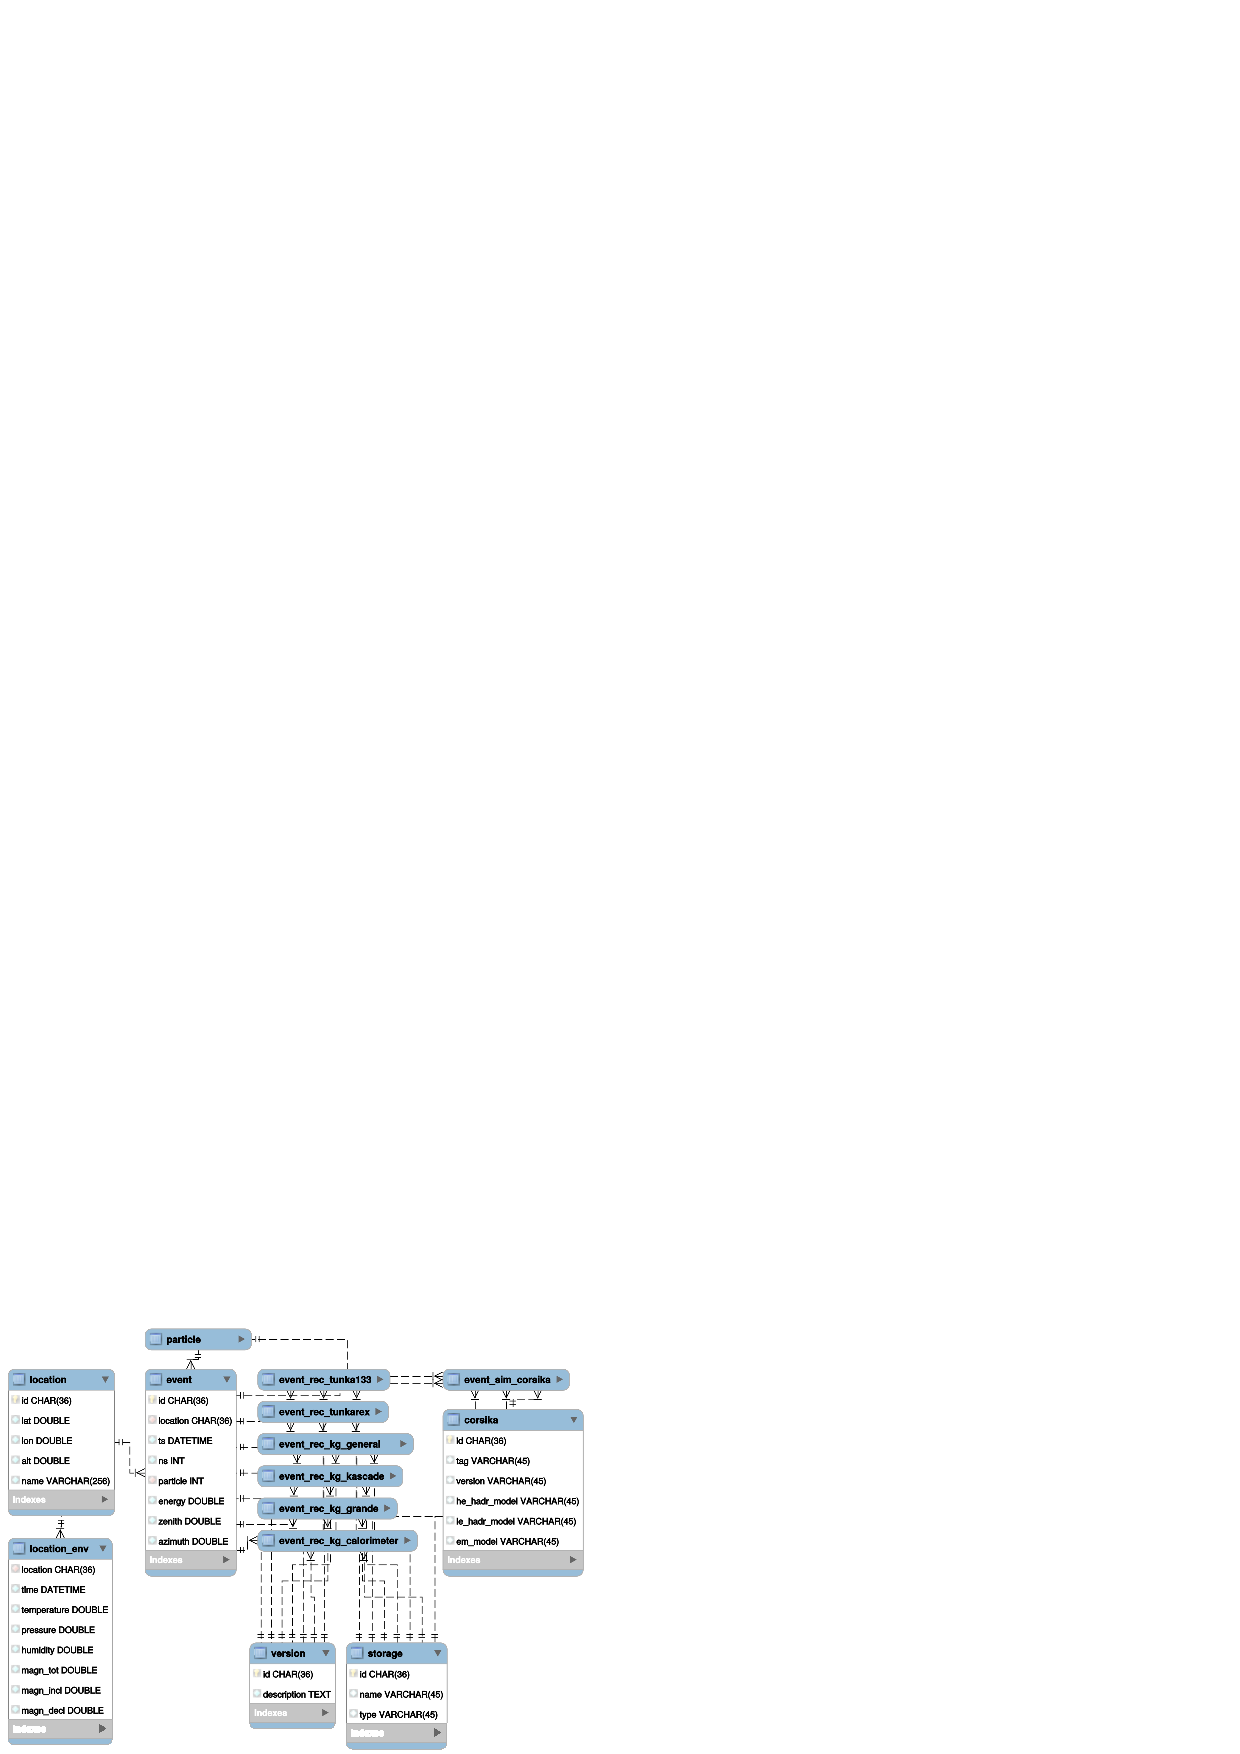
\includegraphics[width=0.82\textwidth]{pics/metadata.pdf}
    \end{center}
\end{frame}

%Data workflows
% \begin{frame}{Data workflow}
%     \vspace{-2em}
%     \centering
%     \only<1>{\includegraphics[width=1\textwidth]{pics/KRAD_workflow_curr.pdf}}
%     \only<2>{\includegraphics[width=1\textwidth]{pics/KRAD_workflow_hori.pdf}}
% \end{frame}

% TODO:
%         Data summary and challenges (no slide so far :-( )
%         Possible solutions (postgres, cvmfs, etc...)

% APPLICATION SERVER: 
% Application server: 
%         TODO: conception of the aggregation server!!! 
%         computing sources (TODO: which sources can we use to run our application in parallel?)

\begin{frame}{Application server concept in GRADLC}
\textbf{Aim}: to provide user the opportunity to analyze the data selected remotely.

\textbf{Computing sources}: CR local network, clusters (GRIDKa, BW-HPC, etc.), external clouds (Exoscale, OpenNebula, Amazon, Google, etc.).

\textbf{Possible solutions}: 
  \begin{itemize}
    \item HTCondor or HTCondor-based workload management systems: VCondor, Panda, Dirac;
    \item Data mapping plugins;
    \item Metadata DB for faster search;
    \item Data caching on aggregation server
  \end{itemize}

\end{frame}

%  ANALYSIS 
% \begin{frame}{Analysis use-cases}
%     \includegraphics[width=1\textwidth]{pics/an_steps.pdf}
%     \vspace{2em}
%     \begin{itemize}
%         \item Analysis could be either algorithmic or machine learning;
%         \item Machine learning requires large enough statistics\\in order to work properly.
%     \end{itemize}
% \end{frame}

% \begin{frame}{Analysis features}
% \vspace{-3em}
% \begin{block}{Software for data analysis depends on a particular experiment}
%   \begin{itemize}
%     \item Problem: It may even require dedicated system environment
%     \item \textbf{Solution: Virtualization\footnotemark[2]}
%   \end{itemize}
% \end{block}

% \begin{block}{Data analysis requires huge amounts of input data}
%   \begin{itemize}
%     \item Problem: It is often more optimal to perform it on the same site the data are stored
%     \item \textbf{Solution: Job management}
%   \end{itemize}
% \end{block}
% \insimg{ADLC1.pdf}
%   \footnotesize\footnotetext[2]{``The act of creating a virtual (rather than actual)
%   version of something,\\ \hspace{1.5em}including virtual computer hardware platforms,
%   storage devices,\\ \hspace{1.5em}and computer network resources''. $\copyright$ Wikipedia}
% \end{frame}

% %TODO: POSSIBLE SOLUTIONS
% \begin{frame}{Possible solutions \\for the application level}
%  
% \end{frame}


%PHYSICS
% \begin{frame}{Example: stacked analysis of high-energetic gamma rays}
%  \textcolor{red}{there will be some physics soon!}
% \end{frame}

% %CONCLUSION
\section{Conclusion}

\begin{frame}{Open access and education}
    \vspace{-4em}
    \begin{itemize}
        \item Open access: a dedicated portal planned
        \item Education: \textcolor{blue}{\texttt{astroparticle.online}}
    \end{itemize}
    \centering
    \includegraphics[width=0.85\textwidth]{pics/astro_onl.png}
\end{frame}

\begin{frame}{Outlook}
\textcolor{red}{Translate the bullets (in comments) to English!!!}
    \begin{itemize}
    \item mdl
    \item kcdc
%     \item Нужны инструменты совместного доступа к данным различных экспериментов и эффективный бережный менеджмент этих больших объемов данных
%     \item Консоциум gradlc предлагает концепцию дата инжиниринга в области астропартикл физикс, основанный на уже kcdc. 
%     \item В данный момент производятся работы по созданию aggregation data server'a и совместному анализу данных из экспериментов kascade и taiga;
% \item Доступ к ресурса проекта на данный момент частично предоставлен через портал astroparticle.online.
    \end{itemize}
\end{frame}

% \subsection{The end}
% \begin{frame}{}
%     \begin{center}
%         \textcolor{kit-green100}{\Huge Thank you\\for your attention!\vspace{1em}}  
%         \Large Any questions?
%     \end{center}
% \end{frame}


%BACKUP SLIDES
%Appendix: detailed information on collaboration and links to the main sources

% \appendix
% \beginbackup
\section{Appendix}
\subsection{Collaboration}
\begin{frame}[allowframebreaks]
{The German-Russian Astroparticle Data Life Cycle collaboration}
\parbox{0.35\textwidth}{
  \centering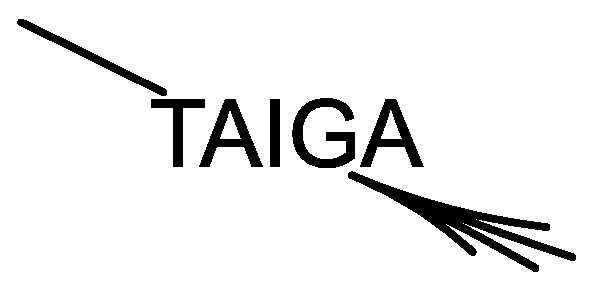
\includegraphics[width=0.25\textwidth]{pics/taiga.eps}
}\hfill
\parbox{0.60\textwidth}{
  TAIGA---Tunka Advanced Instrument for cosmic ray physics and Gamma Astronomy (see
%       https://
  taiga-experiment.info);
}
\\\vspace{1em}
\parbox{0.35\textwidth}{
  \centering
\includegraphics[width=0.35\textwidth]{pics/grande.pdf}
}\hfill
\parbox{0.60\textwidth}{
  KASCADE-Grande---KArlsruhe Shower Core and Array DEtector---Grande\\ (see
%       http://
  www-ik.fzk.de/KASCADE\_home.html);
}
\\\vspace{1em}
\parbox{0.35\textwidth}{
  \centering\includegraphics[width=0.30\textwidth]{pics/Logo_KIT_IKP.pdf}
}\hfill
\parbox{0.60\textwidth}{
  KIT-IKP---Institute for Nuclear Physics Karlsruhe Institute of Technology
}
\\\vspace{1em}
\parbox{0.35\textwidth}{
  \centering\includegraphics[width=0.15\textwidth]{pics/SCC-Logo.png}
}\hfill
\parbox{0.60\textwidth}{
  SCC---Steinbuch Centre for Computing Karlsruhe Institute of Technology
}
\\\vspace{1em}
\parbox{0.20\textwidth}{
  \centering
\includegraphics[width=0.20\textwidth]{pics/SINP_MSU_LOGO.pdf}
}\hfill
\parbox{0.75\textwidth}{
  SINP MSU---Skobeltsyn Institute Of Nuclear Physics Lomonosov Moscow State University
}
\\\vspace{1em}
\parbox{0.20\textwidth}{
  \centering\includegraphics[width=0.15\textwidth]{pics/isu_logo.png}
}\hfill
\parbox{0.75\textwidth}{
  ISU---Irkutsk State University
}
\\\vspace{1em}
\parbox{0.20\textwidth}{
  \centering\includegraphics[width=0.18\textwidth]{pics/matr_logo.png}
}\hfill
\parbox{0.75\textwidth}{
  ISDCT---Matrosov Institute for System Dynamics and Control Theory
}
\end{frame}

\subsection{References}
    \begin{frame}{References}
        \begin{itemize}
            \item Berghöfer T., Agrafioti I. \textit{et al.} Towards a model for computing in European astroparticle physics,
            Astroparticle Physics European Coordination committee, 2016,
            web-source:~\texttt{http://appec.org/wp-content/uploads/\\Documents/Docs-from-old-site/AModelForComputing-2.pdf};
            \item KCDC---\textbf{K}ASCADE \textbf{C}osmic Ray \textbf{D}ata \textbf{C}enter,\\
            web-source:~\texttt{http://kcdc.ikp.kit.edu};
            \item KASCADE-Grande official site, web-source:~\texttt{http://www-ik.fzk.de/KASCADE\_home.html};
            \item TAIGA collaboration official site, web-source:~\texttt{http://taiga-experiment.info};
            \item Astroparticle.online---outreach resource, web-source:~\texttt{http://astroparticle.online}.
        \end{itemize}
    \end{frame}
% \backupend

\end{document}
